% !TeX spellcheck = en_GB 
\section{Interlocking}


\begin{figure}
	\centering
	\begin{subfigure}{.49\columnwidth}
		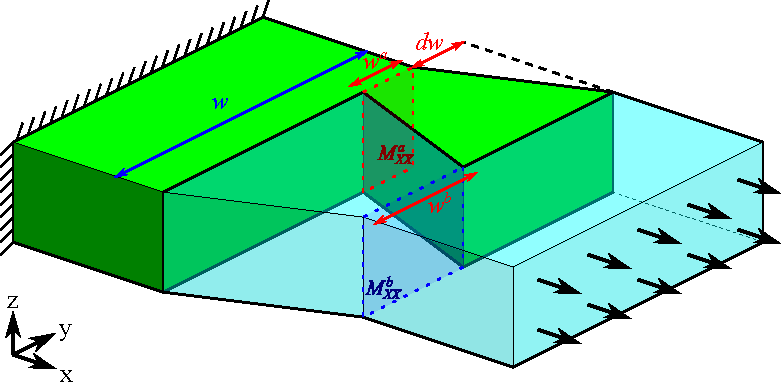
\includegraphics{sources/method/suture_model_v5.pdf}
		\caption{Trapezoidal suture}
		\label{fig:suture}
	\end{subfigure}
	\begin{subfigure}{.49\columnwidth}
		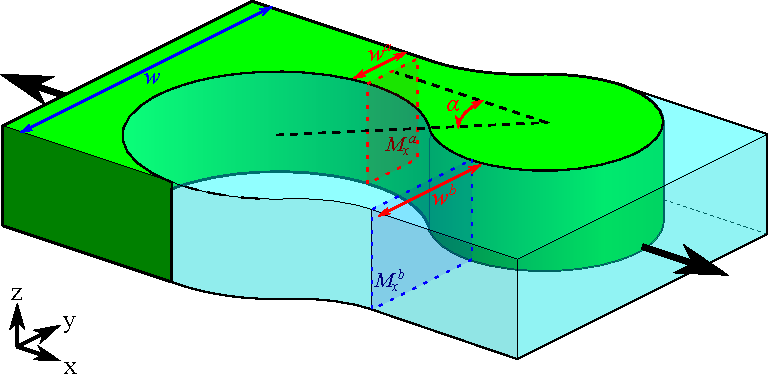
\includegraphics{sources/method/jigsaw_model_v5.pdf}
		\caption{Jigsaw}
		\label{fig:jigsaw}
	\end{subfigure}
	\caption{Simple 2D dovetail interlocking microstructures.}
	\label{fig:suture_jigsaw}
\end{figure}



We will optimize interlocking structures for tensile strength;
the geometry of the designs are optimized to yield or break at the highest horizontally applied tensile stress.
The highest administrable force applied to a unit cell of any interlocking structure will be borne by both materials $a$ and $b$.
At any cross-section perpendicular to the applied stress the total force will be distributed over the area $A_a$ covered by material $a$ and likewise over the area $A_b$.
The best interlocking microstructure will be such that the stress will be homogeneously distributed over $A_a$ and $A_b$ and both will be at the yield strength of their respective base materials:

\begin{align}
	\sigma^* &= \frac{F}{A_\text{total}} = \frac{F}{A_a + A_b}  \nonumber
	= \sigmafail{a} \frac{A_a}{A_a + A_b} \nonumber
	= \sigmafail{b} \frac{A_b}{A_a + A_b} \nonumber \\
%	\sigmafail{a} A_a &= \sigmafail{b} A_b \nonumber \\
\label{eq:general_uper_bound}
	\sigma^* % &= \sigmafail{b} \left(\frac{ \nicefrac{\sigmafail{a}}{\sigmafail{b}} }{ \nicefrac{\sigmafail{a}}{\sigmafail{b}} + 1 } \right) \nonumber \\
	% &= \sigmafail{b} \left(\frac{ 1 }{ 1 + \nicefrac{\sigmafail{b}}{\sigmafail{a}} } \right)  \nonumber \\
	&= \frac{ 1 }{ \nicefrac{1}{\sigmafail{a}} + \nicefrac{1}{\sigmafail{b}} } 
	\approx \SI{8.6}{\mega\pascal}
\end{align}


This upper bound to the ultimate tensile strength of interlocking microstructures is just a theoretical limit.
In practice the worst cross-sectional area $A_a$ is in a different plane than the worst cross-sectional area $A_b$, so they don't add up to $A_\text{total}$.
In the jigsaw example the highest stress of a jigsaw bulb of material $a$ is at its base $\myz{a}$, while the highest stress in $b$ will be at the main body of the bulb of material $a$ at $\myz{b}$.
See \cref{fig:jigsaw}.
The geometry by which the interlock is secured reduces the strength compared to the theoretical upper bound of the ultimate tensile strength.
% Moreover, the stress distribution won't be homogenous when subjecting a complex geometry to tension.




For the materials chosen by this study, Ultimaker Tough PLA (TPLA) and Ultimaker PolyProlylene (PP), the upper bound comes out to be \SI{8.6}{\mega\pascal}.
Because of the layer-wise build-up employed by FDM 3D printing, the tensile properties in the Z direction are different from those in the horizontal plane.
See \cref{tab:mat_props_manufacturing_constraints}.

The structure is furthermore subject to manufacturing constraints determined by the nozzle sizes and the layer thickness.
It should be noted that with a nozzle size of \SI{0.4}{\milli\meter} one can still manufacture geometry as small as \SI{0.3}{\milli\meter}.
In order to generate the correct toolpaths we use the Cura Arachne Engine beta release, which implements the framework for generating variable line width toolpaths from \cite{Kuipers2020}.
\todo{(Make proper reference to Cura?)}


\begin{table}
	\caption{Material properties and manufacturing constraints}
	\label{tab:mat_props_manufacturing_constraints}
	\begin{tabular}{l|rrrr}
		material $m$ & $\sigmafail{m}$ & $\sigmafailz{m}$ & 
		$\wmin{m}$ & $\hmin$ \\
		\hline
		TPLA & \SI{47}{\mega\pascal} & \SI{33}{\mega\pascal} & \SI{0.3}{\milli\meter} & \SI{0.1}{\milli\meter} \\
		PP & \SI{10.5}{\mega\pascal} & \SI{10.6}{\mega\pascal} & \SI{0.3}{\milli\meter} & \SI{0.1}{\milli\meter}
	\end{tabular}
\end{table}






\begin{figure}
	\centering
	\begin{subfigure}[B]{.49\columnwidth}
		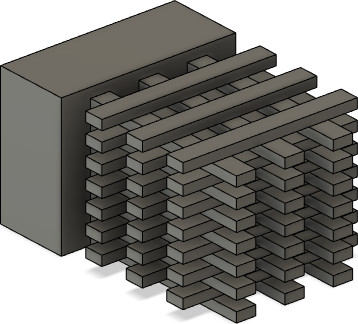
\includegraphics{sources/method/basic_lattice.jpg}
		\caption{The IGIM lattice. (one material shown)}
		\label{fig:basic_structure_single_mat}
	\end{subfigure}
	\begin{subfigure}[B]{.49\columnwidth}
		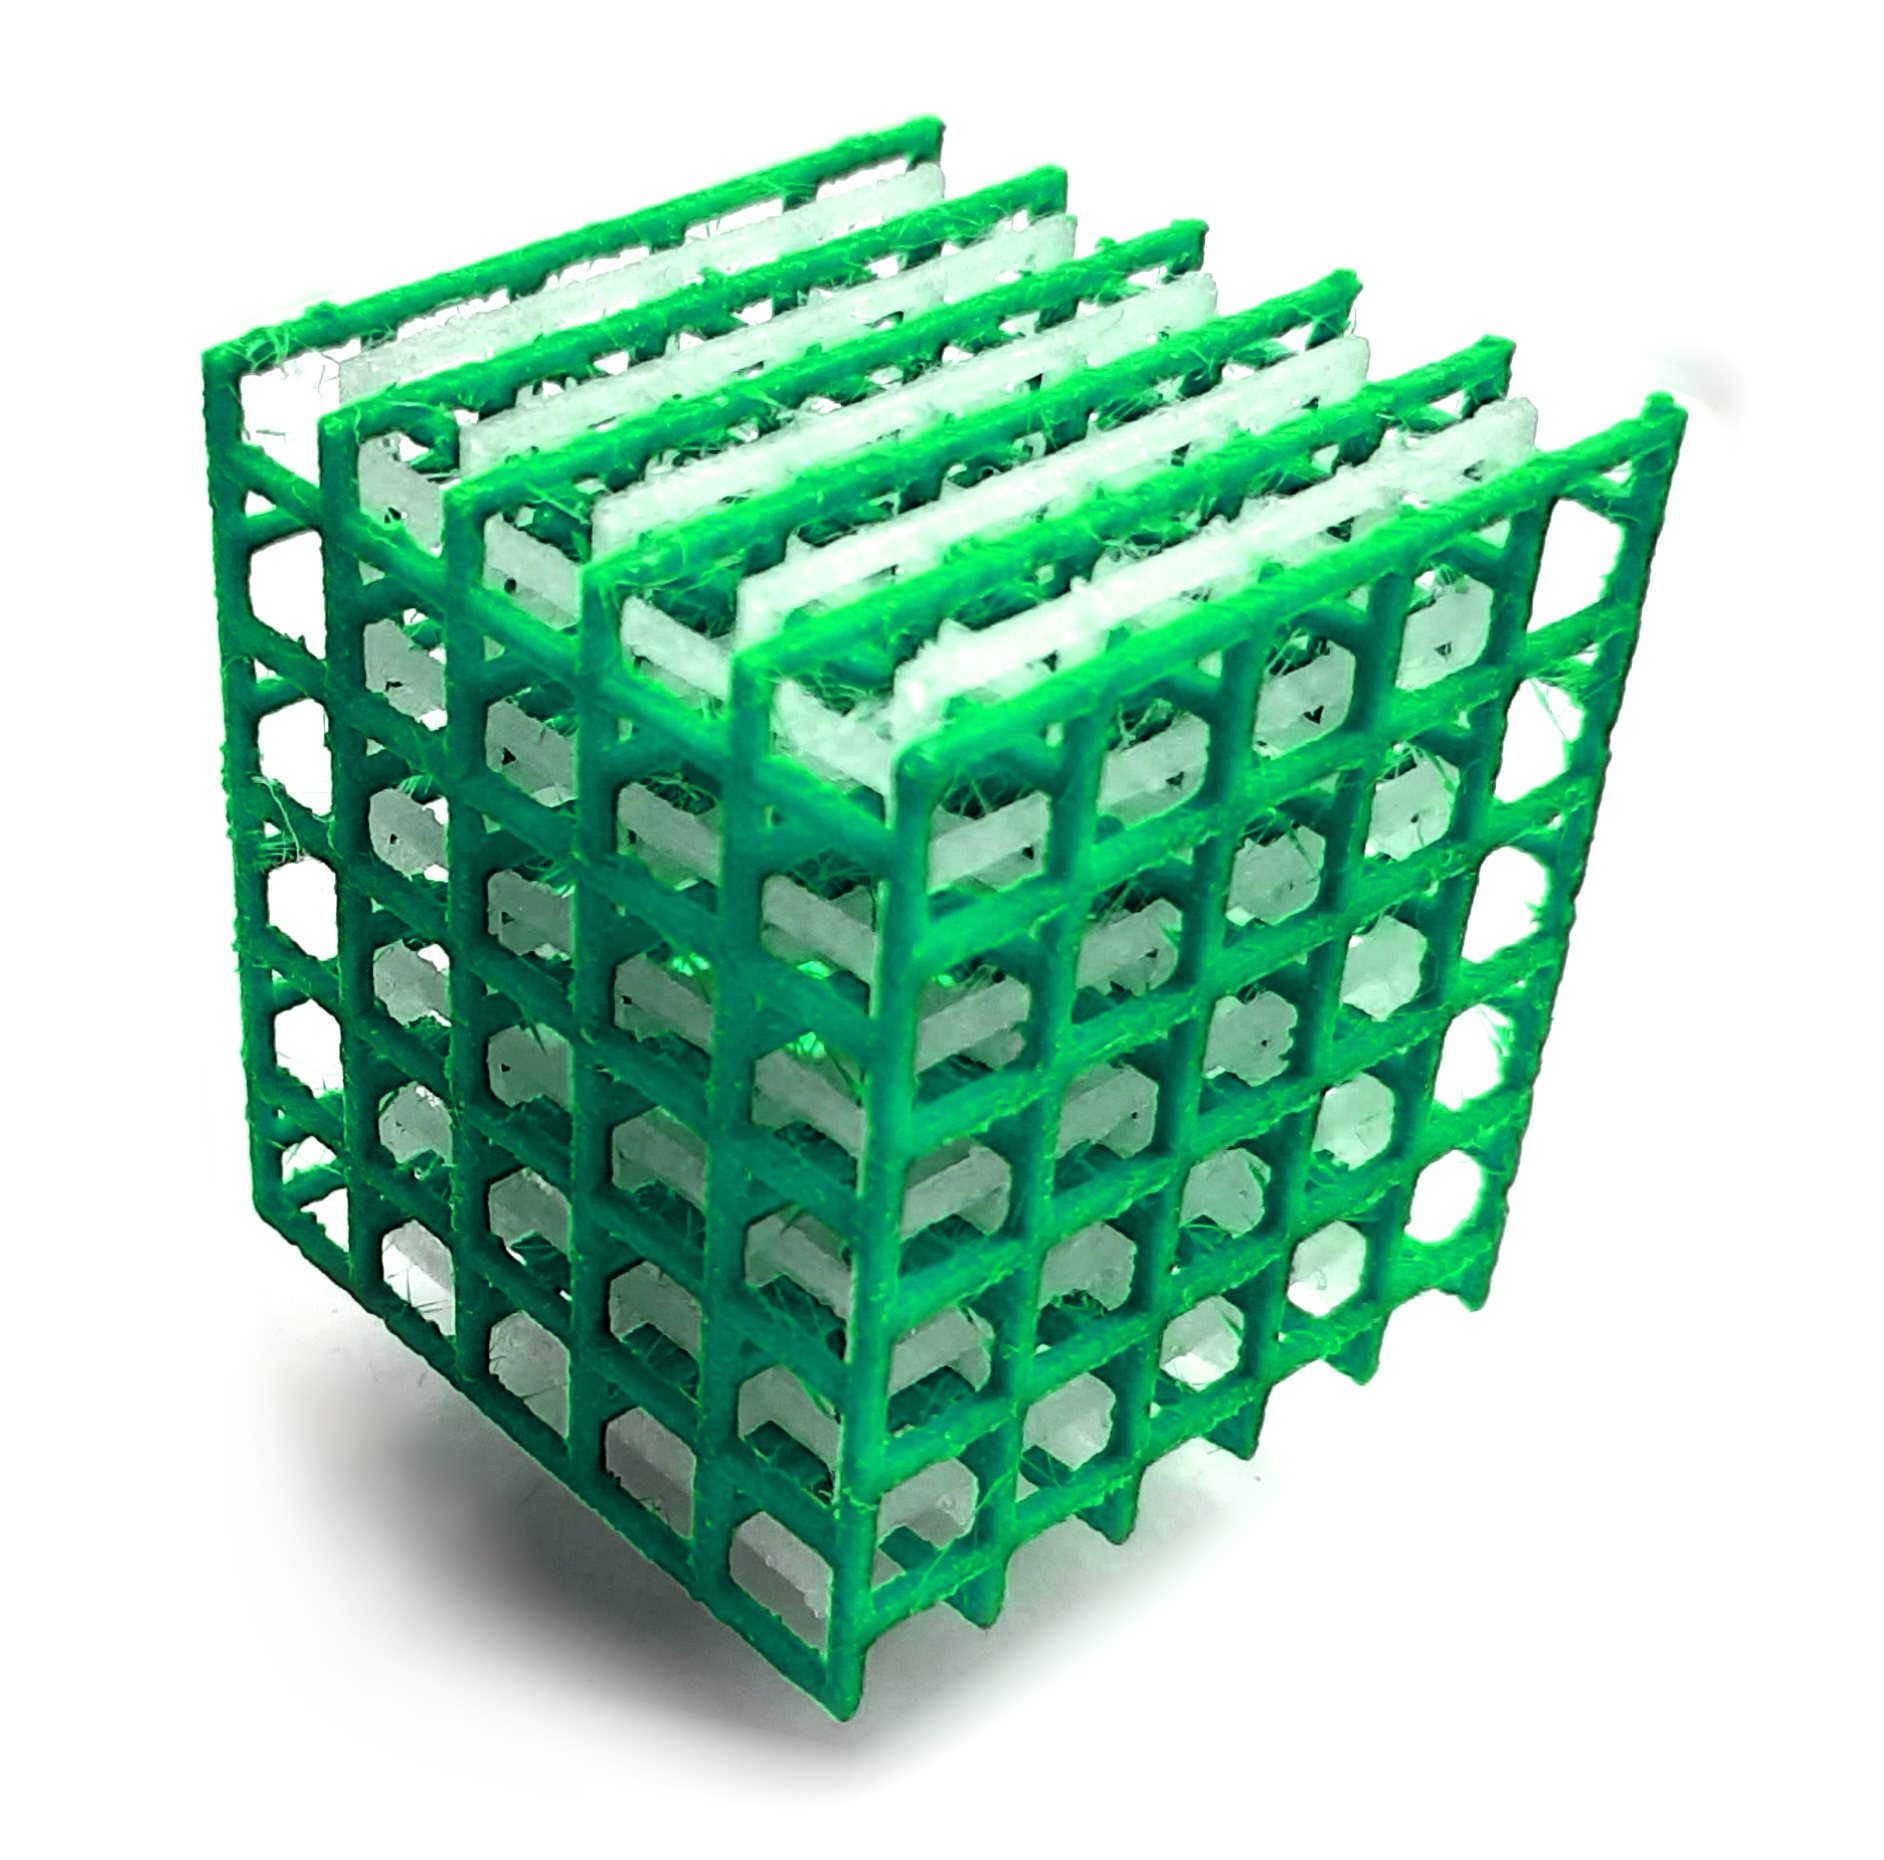
\includegraphics{sources/method/connectivity_lattice.jpg}
		\caption{Connectivity graph}
		\label{fig:connectivity_graph}
	\end{subfigure}
	%\caption{}
	\label{fig:basic_structure}
\end{figure}


\section{Interlaced Genus Interlocking Microstructure}
The genus interlocking structure we propose consists of horizontal beams alternating in material.
On top of that we print another set of beams rotated about Z.
Long horizontal beams assure continuous extrusion, while the alternating direction of the beams assures the interlock - simple and effective.
See \cref{fig:basic_structure}.

When joining bodies of a different material, some region around the interface between the two bodies would be replaced by such a lattice structure.
The interface could be several cells wide, but if the beams were of constant width then the addition of extra cells wouldn't increase the tensile strength of the interface lattice.
One might consider varying the width of the beams in order to optimize the tensile strength.
Each added cell would increase the tensile strength, but by a lesser degree than the last added cell.
In practice the amount of space available is limited by the design of the two bodies.
We consider a design constraint of $\lmax = 3.6$.

Given such a design constraint the efficacy of adding extra cells in the direction of the applied force is weighed against widening the beams.
Instead of having multiple cells with a fraction of the $\lmax$ width it's better to make a single cell as wide as $\lmax$.
Verifying this conjecture falls outside the scope of this work.

Given that we will fill the space around the interface with a single layer of cells, the orientation of those cells w.r.t. the interface is relevant.
While rotating the lattice about X or Y is impossible due to the continuous extrusion constraint, we are free to rotate about Z.
However, given that the tensile stress is applied in a single direction it only makes sense to consider two orientations: straight and diagonal.
This section considers these two designs and analytical models to optimize them.





\begin{figure}
	\centering
	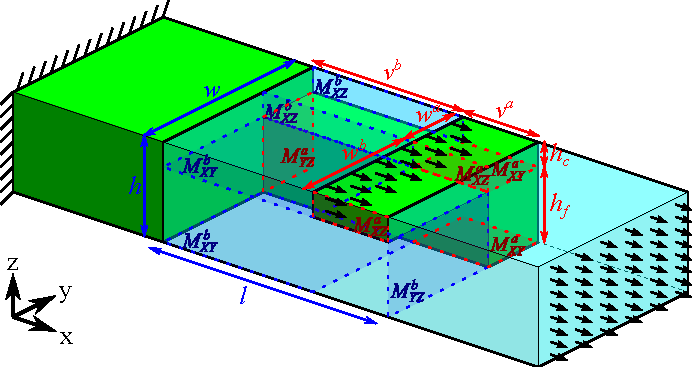
\includegraphics[width=\columnwidth]{sources/method/straight_model_v5.pdf}
	\caption{Straight cell of the IGIM lattice}
	\label{fig:straight_model}
\end{figure}

\subsection{Straight}
The straight model can be seen in \cref{fig:straight_model}.
A cell consists of a single \emph{finger} protruding from the body outward from material $a$ and part of a \emph{cross beam} angled at \SI{90}{\degree}.
In order to print the relatively short fingers using continuous extrusion, we employ the constraint that $\wm \ge 2\wmin{m}$,
whereas the cross beams are long and continuous enough, so $\vm \ge \wmin{m}$.
We set the minimum height of either of the beams to twice the layer height, so as to be able to recover from manufacturing inaccuracies: $\hf \ge \hmin$ and $\hc \ge \hmin$.
\footnote{If the structure would consist of alternating geometry each layer, then the inaccuracy of the one layer can cause overextrusion in the next layer, which escalates the problem upward.}

The total tensile strength of the microstructure is given by $\nicefrac{F}{(\wa +\wb)(\hf + \hc)}$.
Because the objective and all stresses are invariant under scaling,
we can safely assert that a subset of the bounds on the design variables are met, in order to limit the design space from six to three dimensions:
\begin{align*}
	\wa &= 2 \wmin{a} \\
	\hc &= \hmin \\
	\va &= \lmax - \vb
\end{align*}

A careful analysis of the geometry will show that if shearing failure mode $\myz{a}$ has occurred, 
there is still interlocking between the two materials. 
If a part of the cross beams of $a$ has sheared off, still a column of material $a$ remains, which is surrounded by material $b$.
Once failure mode $\myz{a}$ has occurred, still any other failure mode has to occur for the interlock to fail.
Since the Young's modulus of PP is lower than that of TPLA, we know that $\myz{a}$ will always happen before $\myz{b}$.
We will therefore construct two models: one where the TPLA cross beam is whole and one where it is broken into segments.

\subsubsection{Whole cross beams}
In order to optimize it for a maximal tensile strength we consider three types of stress, related to three types of failure mode for either material $m$:
tensile stress $\stresstensile{m}$ for $\myz{m}$, cross beam shear stress $\stresscrossshear{m}$ for $\mxz{m}$ and Z shear stress $\stresszshear{m}$ for $\mxy{m}$.
These three failure modes are modelled as having a homogenous stress distribution:

\begin{align}
	\stresstensile{m} &= \frac{ F }{ \wm \hf } \label{eq:tensile} \\
	\stresscrossshear{m} &= \frac{\w{\neg m}}{w} \frac{ F}{2 \vm \hc} \label{eq:cross_shear} \\
	%	\stresszshear{m} &= \frac{\sigmafail{m}}{\sigmafailz{m}} \frac{\w{m}}{w}  \frac{ F }{ 2 \vm \wm} \label{eq:z_shear} \\
	\stresszshear{m} &= \frac{\w{m}}{w}  \frac{ F }{ 2 \vm \wm} \label{eq:z_shear} \\
	\text{where } & m \in \left\{ a, b \right\} \text{ and } \neg a = b \text{ and } \neg b = a  \nonumber
\end{align}

Because the total force $F$ is modelled as being homogeneously distributed over the whole cross beam,
the two shear stresses obtain only a portion of the total force.
The shear stress is multiplied by one half because the beams are fixed on both sides.
%The Z shear stress $\stresszshear{m}$ is multiplied with the ratio between the vertical and horizontal strength, so that all stresses can be compared to $\sigmafail{m}$ fairly.

The above considerations combine to form the following constrained optimization problem:

\begin{align}
	f: & \min{ \frac{\left( 2 \wmin{a} + \wb \right) \left( \hf + 2\hmin \right) }{F} }\\
	\omit\rlap{subject to} \nonumber \\
	\gwb: & 1 - \nicefrac{\wb }{2 \wmin{b}} \le 0 		&&	\text{ Nozzle size} \label{eq:gwb}\\
	\gva: & 1 - \nicefrac{ \left( \lmax - \vb \right) }{\wmin{a}} \le 0 		&&	\text{ Nozzle size} \label{eq:gva}\\
	\gvb: & 1 - \nicefrac{\vb }{\wmin{b}} \le 0 		&&	\text{ Nozzle size} \label{eq:gvb}\\
	\ghf: & 1 - \nicefrac{\hf}{\hmin} \le 0 		&&	\text{ Layer thickness } \label{eq:ghf}\\
	\gta: & 1 - \frac{ 2 \wmin{a} \hf \sigmafail{a} }{ F } \le 0 &&	\text{ Tension failure } \myz{a}  \label{eq:g_tensile_a} \\
	\gtb: & 1 - \frac{ \wb \hf \sigmafail{b} }{ F } \le 0 &&	\text{ Tension failure } \myz{b}  \label{eq:g_tensile_b} \\
	\gca: & 1 - \frac{ 2 w \left( \lmax - \vb \right) 2 \hmin \sigmafailz{a} }{ \wb F \sqrt{3} } \le 0 &&		\text{ Shear failure } \mxz{a}  \label{eq:g_shear_a} \\
%	\gcb: & 1 - \frac{ 2 w \vb \hc \sigmafailz{b} }{ \wa F \sqrt{3} } \le 0 &&		\text{ Shear failure } M_{\text{y}, b}  \label{eq:g_shear_b} \\
	\gza: & 1 - \frac{ 2 w \left( \lmax - \vb \right) \wa \sigmafailz{a} }{ \wa F \sqrt{3} } \le 0 	&&	\text{ Shear failure } \mxy{a} \label{eq:g_z_shear_a} \\
	\gzb: & 1 - \frac{ 2 w \vb \wb \sigmafailz{b} }{ \wb F \sqrt{3} } \le 0 	&&	\text{ Shear failure } \mxy{b} \label{eq:g_z_shear_b} 
\end{align}

The $\sqrt{3}$ comes from the von Mises yield criterion.
Although one might consider combining the stresses together using the same criterion, this does not increase the accuracy of the model,
because the failure mode planes do not overlap.



inversion; response surfaces; active constraints

\subsubsection{Broken cross beams}


changed problem definition




\subsection{Diagonal}
symmetry; design variables

Manufacturability;Rounded edges with radius $r$

formula for width
\begin{align}
	d &= 2Mw / \sqrt{4M^2-w^2} \\
	M &= L - 2r \\
	w &= \wa + \wb
\end{align}

area of Z shear
\begin{align}
	A_z &= \frac12 \pi r^2 + r (\wa-2r) \frac{d}{w} + d M \left(\frac{\wa}{w}\right)^2
\end{align}


difficult to model; homogeneous stress distribution assumption violated; deformation dependent

assume homogenous tensile stress as if beam was straight?
